\expandafter\ifx\csname ifdraft\endcsname\relax
    %!TEX encoding = UTF-8
% +++
% latex = "uplatex"
% +++
\documentclass[uplatex,dvipdfmx,b5j,openany]{jsbook}
\usepackage{graphicx}

\usepackage{siunitx}		%for use si unit
\usepackage{here}			%for use figure here
\usepackage{tikz}			%for use TikZ package
\usepackage{pgfplots}		%for use PGFplots
\usepackage{dcolumn}		%for use significant figures in the table
\usepackage{csvsimple}		%for import csv files
\usepackage[RPvoltages,americanresistors,americaninductors,europeanvoltage,americancurrents]{circuitikz}
\usepackage[noto]{pxchfon}	%for use Noto fonts

% To out put TikZ logo
\usepackage{bxtexlogo}
\bxtexlogoimport{TikZ}

\usepackage{wrapfig}
\usepackage[top=1.5cm, bottom=1.5cm, left=2.5cm, right=2cm]{geometry}

% framed settings
\usepackage{framed}
\definecolor{shadecolor}{gray}{0.80}

% mdframed settings
\usepackage[xcolor,framemethod=tikz]{mdframed}
\usetikzlibrary{shadows}
\mdfdefinestyle{bash}{linecolor=black,linewidth=0.5pt}
\mdfdefinestyle{shadow}{linewidth=0pt,backgroundcolor=black!15}

\usepackage[customcolors]{hf-tikz}
\hfsetfillcolor{black!5}
\hfsetbordercolor{black!50}

\usepackage[cache=false]{minted}

\usepackage{uri}

\tikzset{% tikz style set
  	pointtype triangle/.style={mark=triangle*,mark size=4pt},
  	every mark/.style={fill=white,solid},
  	south west label/.style={
		matrix,matrix of nodes,
		anchor=south west,at={(rel axis cs:0.01,0.01)},
		nodes={anchor=west,inner sep=0},
  	},
}

\pgfplotsset{% graph style set
    table/col sep=comma, % Use CSV files
  	compat=1.12,
  	major tick length=0.2cm,
  	minor tick length=0.1cm,
  	every axis/.style={semithick},
  	tick style={semithick,black},
  	legend cell align=left,
  	legend image code/.code={%
		\draw[mark repeat=2,mark phase=2,#1]
	  	plot coordinates {(0cm,0cm) (0.5cm,0cm) (1.0cm,0cm)};
  	},
  	log number format basis/.code 2 args={
	\pgfmathsetmacro\e{#2}
	\pgfmathparse{#2==0}\ifnum\pgfmathresult>0{1}\else
	\pgfmathparse{#2==1}\ifnum\pgfmathresult>0{10}\else
	{$#1^{\pgfmathprintnumber{\e}}$}\fi\fi},
}

% macros
\newcommand{\logoLaTeX}{{\rm \textbf \LaTeX}\hspace{0zw}}
    \graphicspath{{./figure/}}
\begin{document}
\fi

\chapter{環境構築と初期設定}
	\LaTeX を使うにあたり最も大きな障壁とされるのが環境構築\footnote{そのソフトを使える環境を整えること}と言われています。
	確かにMicrosoft Wordなどと比べれば導入は少々煩雑ではありますが、
	多くの方々の尽力により今ではとても簡単になっているので、身構えることはありません。

	\section{\LaTeX を使うのに必要なもの}
		まず、\LaTeX のソフトそのものが必要になりますが、\LaTeX は単体のソフトウェアではなく、多くの関連ソフトの集合体です。
		それらを一つ一つ導入していくのはとても手間がかかるので、
		\LaTeX では関連するソフトをひとまとまりにした状態で配布するディストリビューションという形態がとられています。
		現在配布されているディストリビューションにも数種類あるのですが、
		現在最もポピュラーな\TeX Liveというディストリビューションを今回使用します。

		また\LaTeX は、マークアップ言語と呼ばれるプログラミング言語のような形で文章の構造を指定します。
		そのため\LaTeX を使うためには\LaTeX 本体ソフトウェア以外にもマークアップ言語を記述するためのテキストエディタが必要になります。
		\TeX Liveにも一応\TeX Worksというテキストエディタが同梱されているのですが、お世辞にもモダンとは言えません。
		ですので、今現在\LaTeX に限らず多くのプログラミング言語の開発環境に用いられているVisual Studio Codeというエディタを使用します。

		今回インストールするソフトウェアは以下の2つとなります。
		\begin{description}
			\item[\LaTeX ディストリビューション] \TeX Live
			\item[テキストエディタ] Visual Studio Code
		\end{description}
		これらのソフトウェアの導入手順を以下にて解説します。

	\section{\TeX Liveの導入}
		まず最初に\TeX Liveを導入します。

		\subsection{Windows}
			以下のページよりネットワークインストーラをダウンロードします。	\\
			\url{https://www.tug.org/texlive/acquire-netinstall.html}	\\
			このページを開いて、\url{install-tl-windows.exe}をダウンロードします。

			\begin{wrapfigure}{r}[0pt]{0.5\textwidth}
				\centering
				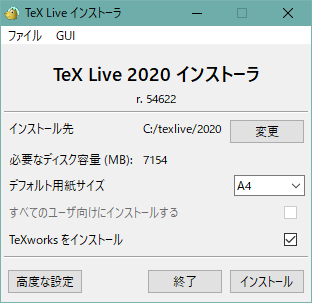
\includegraphics[width=5cm]{TeXlive-installer2.png}
			\end{wrapfigure}
			
			ダウンロードしたファイルを起動すると展開用のソフトが起動するので、installを選択し次に進み、installボタンを押下します。
			すると右のようなインストーラが起動します。
			ここで様々なインストールの設定が行えますが、たいていの場合変更は必要ありません。
			インストール先もここの設定で変更が可能ですが、本書では変更しないという前提で解説をします。
			
			インストールボタンを押下するとインストールが開始されます。
			かなり時間がかかるので放置しておきます。

			終わったらインストーラを閉じてインストールは完了です。

		\subsection{Linux}
			パッケージ管理ソフトを使用するのでまず最初に更新を行います。\\
			apt(Debian,Ubuntuなど)では以下のように
			\begin{mdframed}[linecolor=black,linewidth=0.5pt]
				\begin{verbatim}
					$ sudo apt update
					$ sudo apt upgrade
				\end{verbatim}
			\end{mdframed}
			pacman(Arch Linuxなど)では以下のようにします。
			\begin{mdframed}[linecolor=black,linewidth=0.5pt]
				\begin{verbatim}
					$ sudo pacman -Syu
				\end{verbatim}
			\end{mdframed}

			\expandafter\ifx\csname ifdraft\endcsname\relax
\end{document}
\fi